\newpage
\section{Coloreo}

Un \emph{``coloreo''} de los v\'ertices de un grafo $G = (V, E)$ es una asignaci\'on $f : V \rightarrow C$, tal que $f(v) \neq f(w)$ para todo $(v,w) \in E$. Para todo entero positivo $k$, un \emph{``$k$-coloreo''} de $G$ es un coloreo que usa exactamente $k$ colores.

\raggedright
\bigskip
\begin{center}
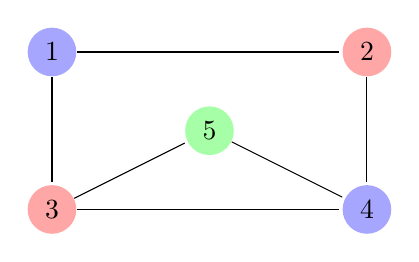
\begin{tikzpicture}[shorten >=1pt, auto, node distance=3cm,
  vertex_red/.style={fill=red!35, circle},
  vertex_green/.style={fill=green!35, circle},
  vertex_blue/.style={fill=blue!35, circle}]

\node[vertex_blue] (n1) at (-7,1)  {1};
\node[vertex_red] (n2) at (-3,1)  {2};
\node[vertex_red] (n3) at (-7,-1)  {3};
\node[vertex_blue] (n4) at (-3,-1)  {4};
\node[vertex_green] (n5) at (-5,0)  {5};


\draw(n2) -- (n4);
\draw(n1) -- (n3);
\draw(n1) -- (n2);
\draw(n3) -- (n5);
\draw(n3) -- (n4);
\draw(n5) -- (n4);

\end{tikzpicture}
\end{center}
\raggedright
\bigskip

Un grafo se dice \emph{``$k$-coloreable''} si existe un $k$-coloreo de $G$. De esta manera definimos al n\'umero crom\'atico de $G$, $\chi(G)$, como el menor n\'umero de colores necesarios para colorear los v\'ertices de $G$. Un grafo se dice \emph{``$k$-crom\'atico''} si $\chi(G) = k$. Notar que el grafo de la figura es $3$-crom\'atico.

Algunos ejemplos:

\begin{itemize}
\item $\chi(K_n) = n$
\item Si $G$ es planar $\Rightarrow \chi(G) = 4$\footnote{Teorema de los Cuatro Colores}
\item Si $G$ es bipartito $\Rightarrow \chi(G) = 2$
\item Si $C_{2k}$ es un circuito simple par $\Rightarrow \chi(C_{2k}) = 2$
\item Si $C_{2k+1}$ es un circuito simple impar $\Rightarrow \chi(C_{2k+1}) = 3$\
\end{itemize}


\subsection{Cotas para $\chi(G)$}
\begin{itemize}
\item Si $\Delta(G)$ es el grado m\'aximo de $G$, entonces $\chi(G) \leq \Delta(G) + 1$.
\item Si $G$ es un grafo conexo que no es un circuito impar ni un grafo completo, entonces $\chi(G) \leq \Delta(G)$\footnote{Teorema de Brooks}.
\item Si $H$ es un subgrafo de $G$, entonces $\chi(H) \leq \chi(G)$.
\item $\omega(G) \leq \chi(G)$\footnote{Una \emph{``clique''} es un subgrafo completo maximal de un grafo. El \emph{``n\'umero clique''} de un grafo es el m\'aximo n\'umero de v\'ertices de una clique de $G$, y se denota por $\omega(G)$.}.
\end{itemize}


%\subsection{Teorema de Heawood (1890)}
%Si $G$ es un grafo planar, entonces $\chi(G) \leq 5$.

\newpage
\subsection{Algoritmos para coloreo de grafos}

Dado un grafo $G$ de $|V|$ v\'ertices y un entero $k$, el problema de decisi\'on que consiste en determinar si existe un $k$-coloreo para $G$ es NP-completo, y su complejidad es  $\mathcal{O}(2^{|V|} * |V|)$.

Dado un grafo $G$ de $n$ v\'ertices y un entero $k$, el problema de decisi\'on que consiste en determinar si $\chi(G) = k$ es NP-Hard.

\begin{itemize}
\item \textbf{Heur\'istica secuencial (S)}: Dado un orden $v_1, v_2, ..., v_{|V|}$ de $V$, asignar en el paso $i$ el menor color posible a $v_i$. Es decir, el color m\'as chico que no est\'a siendo usado por los vecinos de $v_i$ (greedy). Puede devolver resultados bastante malos en algunos grafos.
\item \textbf{Algoritmo secuencial con backtracking (exacto)}: La idea es ir asignado colores uno por uno a los diferentes v\'ertices, arrancando desde el v\'ertice 0. Antes de asignar un color, miramos los colores de los vecinos de dicho v\'ertice. Si encontramos un color apropiado, se lo ponemos al v\'ertice en cuesti\'on. Si no es posible encontrar un color apropiado, volvemos hacia atr\'as y probamos con otro color en alg\'un v\'ertice anterior.
\end{itemize}

\subsection{Polinomio crom\'atico}

Dado un grafo $G$, su \emph{``polinomio crom\'atico''} cuenta las maneras en las cuales puedo colorear a $G$ usando un n\'umero $n$ de colores. Por ejemplo, el polinomio crom\'atico de $K_3$ es $n(n-1)(n-2)$, lo cual significa que si tengo $4$ colores puedo colorear a $K_3$ de $4*3*2=24$ maneras distintas.

\subsection{Grafos perfectos}

Un grafo $G$ es \emph{``perfecto''} si $\chi(H) = \omega(H)$ para todo subgrafo inducido $H$ de $G$. Existe un algoritmo polinomial para determinar $\chi(G)$ si $G$ es perfecto \footnote{Teorema de Grotschel, Lov\'asz y Schrijver}.

Un grafo es perfecto si y s\'olo si su complemento es perfecto. Un grafo es perfecto si y s\'olo si no tiene ciclos impares ni complementos de ciclos impares como subgrafos inducidos.

\subsection{Coloreo de ejes}

Un \emph{``coloreo de ejes''} de un grafo $G$ es una asignaci\'on de colores a los mismos en el cual dos ejes que tienen un v\'ertice en com\'un no pueden tener el mismo color.

El \emph{``\'indice crom\'atico''} $\chi'(G)$ de un grafo $G$ es el menor n\'umero de colores con el que se pueden colorear los ejes de $G$. Para todo grafo $G$ se cumple que $\Delta(G) \leq \chi'(G) \leq \Delta(G) + 1$ \footnote{Teorema de Vizing}.

